\chapter{Testing of MOM}
There are different ways to evaluate the web interface e.g. an expert or user-based evaluation could be made. We would have preferred to make a user-based evaluation because this gives a valuable input from a person who might use the system. However, to make such a sufficient user evaluation then we should find at least people with children which is between 3-12 years old and that would take too much time.\fixme{We could talk about how we tried to get test-users in the beginning of the project.} A user-based evaluation of the entire MOM system would be optimal if the user and his/hers family could try it for a week or two before we interview them about the system. Also a log for our benefit could be made during this time to see how they use it of course with the test persons permission. Therefore we can only evaluate the web interface. For this we use an expert evaluation called Heuristic evaluation. 

\section{Heuristic evaluation in Theory}
In a Heuristic evaluation the test persons look for errors and potential usability errors which can be categorized in 12 item and divided into 3 groups\citep{DIEB}, which is shortly described below:
\begin{description}
\item[Learnability] make it easy for the user to learn and remember the system:
\begin{itemize}
	\item Visibility - make it clear for the user which functions are available in the system and show what the system is doing.
	\item Consistency - be consistent in the design features and let it be similar to other comparable systems
	\item Familiarity - the language and symbols in the system should be familiar to the user.
	\item Affordance -  E.g. if it looks like a button, it is a button. 
\end{itemize}

\item[Effectiveness] is how easy it is for the user to use it and how safe it is to use:
\begin{itemize}
	\item Navigation - provide support to enable people to move around. Make clear navigation instructions.
	\item Control - make it clear who and what is in control, the user should be able to take control. There should be a connection between what happens in the system and what will happen outside of the system. 
	\item Feedback - give feedback on what have happened after user do an action in the system.
	\item Recovery - how good it is to recover if the user makes an error. 
	\item Constraints - prevent people from doing inappropriate things in the system. This should be able to prevent serious error.
\end{itemize}

\item[Accommodation] accommodating differences between and respecting those differences:
\begin{itemize}
	\item Flexibility - let there be multiple ways of doing things.
	\item Style - is the design attractive to the user. 
	\item Conviviality - be polite and friendly. Do not use aggressive language.
\end{itemize}
\end{description}

Typically the test is done by 1-3 test persons\citep{HeuristicEvaluation}. The test person should be a usability expert or a software developer with the expertise in a relevant system. To make the test they should have relevant information of the user and a set of tasks to follow but they are also allowed to make their own.


\section{Heuristic Evaluation of Media-Online Management}
Before performing a Heuristic evaluation we need to determine what is needed before the evaluation is done and how the results should be presented\citep{HeuristicEvaluationGuide}.

\subsection{Planning the Evaluation}
When planing the evaluation the test persons need to get test persons. They need to get a small description of the user and some test cases. They should also get a list of the heuristics from which the system need to be evaluated from. This should all be made prior to the evaluation. \\

The evaluation of Media-online Management system is being done by test persons in the group which have been highly involved in the development of the system. This is not optimal in this test where the test persons should be an usability expert from outside the development group\citep{DIEB}.\\

The test persons also need to know the user. So the test persons need a general description of the user and their technology capabilities. The user of MOM is parents and children. The children is only in contact with the controller and the parents are both using the controller and the website. The parents has a general experience with the internet, but they are not experts. However we expect them to be able to at least set up an e-mail account with Google or Hotmail. The children has few technology skills but we expect our target group to be able to turn on a normal television. \\

Before the test is conducted some test cases should be made by the development team. This should cover several cases in the system such that the test persons is presented to every aspect of the system. The test cases of MOM can be found in section \vref{sec:testcase}.\\ 


We want to primarily be validated on Visibility, Consistency, Control and Feedback which we find to be the more important for the Media online Management system.

\subsection{Presenting the Results}
When presenting the results from the test cases it will be separated in two parts. First the errors and irregularities of the program is presented. Then the Heuristic errors will be presented.\\
Both will use the ranking of severity as is listed below:

\begin{itemize}
    \item Minor - Minor cosmetic or consistency issue.
    \item Moderate - system can succeeded without loss of data but it would course irritation for the user. 
		\item Severe - system losses functionality or data.
    \item Critical - system failure.
\end{itemize}

This ranking can then help priorities and identify the problems that should be corrected first. The results can be found in section \vref{sec:resultHE}.

%testcases
\section{Testcases}
\label{sec:testcase}
In table \ref{tab:testcase} is one of the test cases that we made for testing the entire Media-Online Management. In the test case both a part of the Website and a controller are tested. The changes being done in the web site should affect the controller.\\ 
 All test cases can be found in appendix \vref{appen:testSuite}.
\begin{table}[h]
	\centering
		\begin{tabular*}{\textwidth}{|l|l|}
		\hline
		\hline
		Name: & WS001\\
		\hline
		Description: & \parbox{0.70\textwidth}{Setup a complete system with a managing user, a regular user, a `TV Controller' and the accompanying rights to use it.}\\
		\hline
		Requirements: & \parbox{0.70\textwidth}{
		\begin{itemize}
			\item A computer with Internet access.
			\item The MOM website.
			\item Two Tags prepared with a Tag ID.
			\item An Arduino to function as the TV controller. 
		\end{itemize}}
		\\
		\hline
		Expected Results: & \parbox{.70\textwidth}{Adding of a regular user,tags, a `TV Controller' and the accompanying rights to use it.}\\
		\hline
		Steps: & \parbox{.70\textwidth}{
		\begin{enumerate}
			\item Log into the MOM website with lniel10 and test.
			\item Attach the first Tag to the lniel10 profile.
			\item Add the permissions that enables the use of all devices without expending points.
			\item Create a profile 'Kevin' with 60 points and other appropriate person information to act as a user.
			\item Attach the second tag to Kevin.
			\item Add controller TV into the system.
			\item Add the permissions to log into the TV controller.
			\item Perform Test AT001A on both profiles with addendum: Wait 3 minutes for both users and note if either expends points.
		\end{enumerate}}
		\\		
		\hline
		\end{tabular*}
\end{table}


\section{Collected Results of the Heuristic Evaluation}
\label{sec:resultHE}
In this section we present the errors discovered in connection with the test. The errors have group in to three categories program errors, Heuristic error and other errors and missing functionality.

\subsection{Program Error from Testcases}
Before presenting the results from the test cases it need to be pointed out that during the test some critical errors was discovered and fixed such that the test was able to be completed. The most critical was an error in the validation of whether a valid tag could log-in from a valid controller. Some other error with another severity have also been fixed and they were retested to confirm it. These errors is mentioned in the result and marked as fixed. 

\begin{table}
	\centering
		\begin{tabular}{|p {0.10\textwidth}|p{0.6\textwidth}|p{0.2\textwidth}|p{0.1\textwidth}|}
		\hline
		Test name & The problem &  Rating the severity & Status\\
		\hline
		\parbox{0.10\textwidth}{WS001} & The tag could not activate controller even though it should have access & critical & fixed \\ \hline
		WS002 & Find out how to block a user using a true condition & moderate & unsolved\\ \hline
		WS002 & Adding a rule to block a profile with a true condition, failed & severe & fixed\\ \hline
		WS003 & It was not possible to create a rule to ensure that the media TV is turned on before the media Playstation is able to turn on. In the website there are a form to fill which suggest it can be done, but when saving it an error occurs and it is blaming the user.  & severe & unsolved\\ \hline
		AT001A &  After a user had logged in and out of a controller, this controller would try to log-in again not waiting for a user to swap his tag. & Critical & fixed.\\ \hline
		AT003A & The controller seemed to freeze during the first run of this test but it did not repeat & moderate/minor & unsolved \\ \hline
		AT003C & If a permission has granted access to a media and the parent then deletes this permission then the controller should have cut the power to the media upon next status call to the API, but this did not happen. & moderate & fixed   \\
		\hline
		\end{tabular}
	\caption{Errors found running the testcases}
	\label{tab:ResultsFromTryingOutTheTestcases}
\end{table}

A larger description of the test cases and the results can be found in Appendix \ref{appen:testSuite}.

\subsection{Heuristic Errors}
 Apart from the functionalities tested in the described test cases, all pages in the website have been visited and their functionality tested. When doing this some Heuristic errors has been discovered. As mentioned earlier we prioritize Control, Consistency, Visibility and feedback.


\subsubsection{Consistency}
There are several consistency problem on the website which could cause confusion adn irritation for the user. The errors in it self is only a minor problem but do to the number of errors and their occurrence it is a moderate problem.   

The first example is the add button on the different page that has different coloring and placement compared to the table in which it will be shown. The problem is shown in figure \ref{fig:consistencyButton}.

\begin{figure}
	\centering
		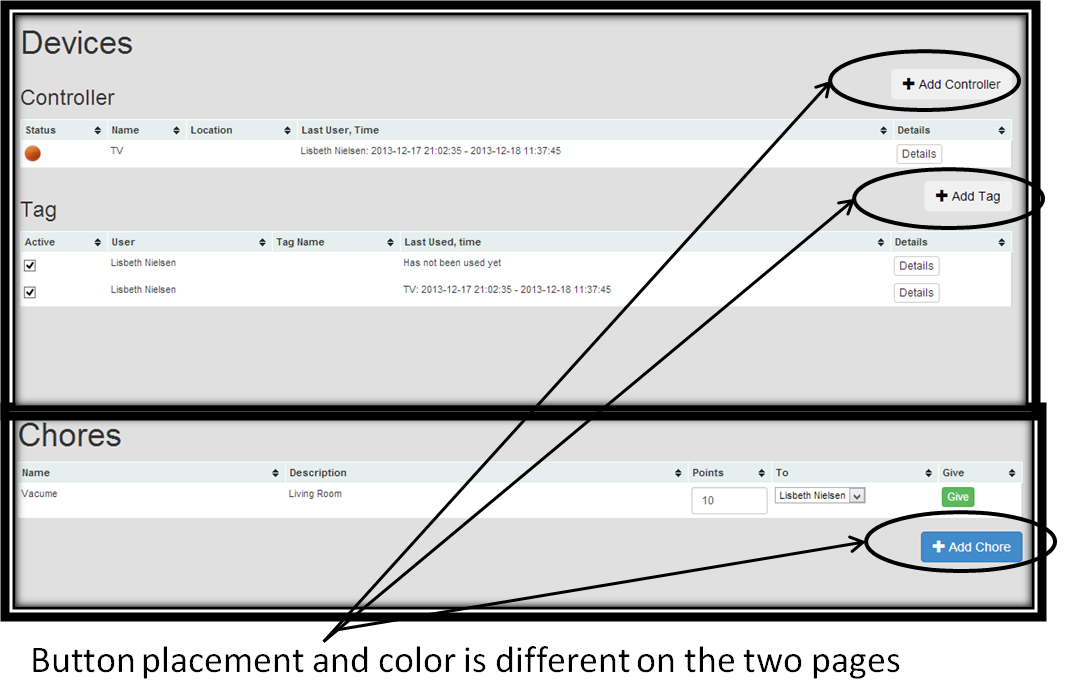
\includegraphics[width=0.75\textwidth]{images/consistencyButton.png}
	\caption{The lack of consistency with buttons}
	\label{fig:consistencyButton}
\end{figure}


Another example is the feedback representation from the system if the user did something wrong, a confirmation message or just a alert for the user. As is shown in figure \ref{fig:afteraddConsistency} there is inconsistencies in where and how the message is provided to the user and it is both feedback after adding something to the system. There are also inconsistencies in where the website redirect the user after adding.

\begin{figure}
	\centering
		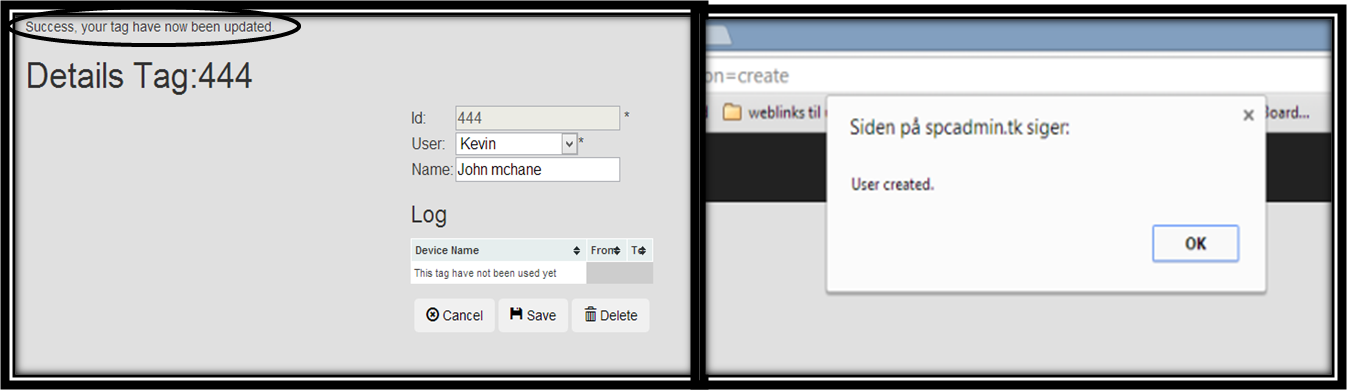
\includegraphics[width=0.75\textwidth]{images/afteraddConsistency.png}
	\caption{Feedback in consistency}
	\label{fig:afteraddConsistency}
\end{figure}

The last example that will be shown is the inconsistency of how the user is guided to fill in the forms when adding something to the system. One method is to indicate it with a \* at the end of the form, which is shown in figure \ref{fig:consistencyAddControllerUser} to the right. The other method is to wait until the user try to save information and then give him an error that he has not filled in the required fields, as shown to the left in the figure. The first alternative is the better to use.

\begin{figure}
	\centering
		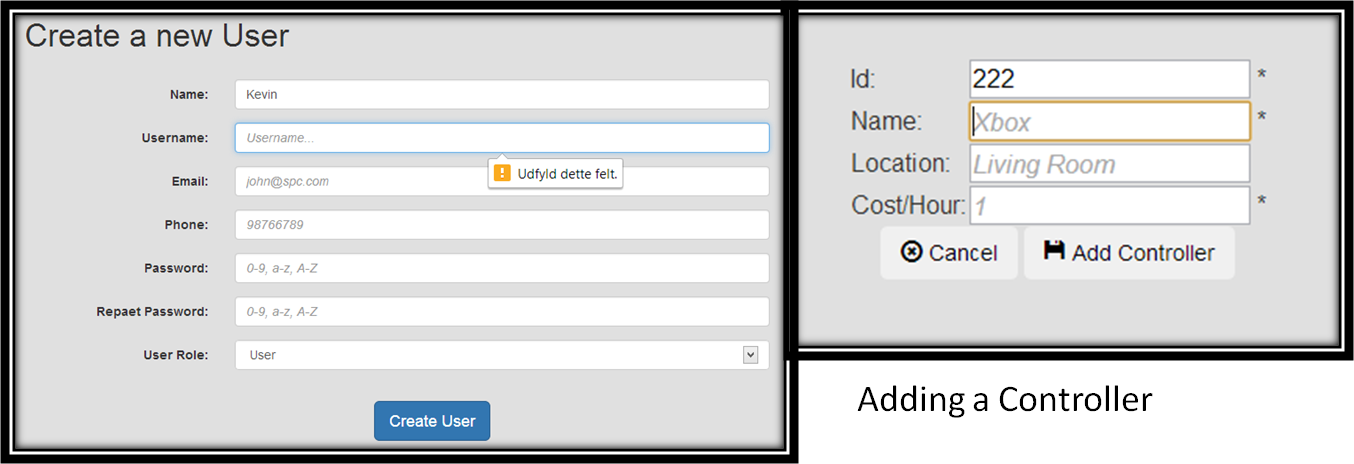
\includegraphics[width=0.75\textwidth]{images/consistencyAddControllerUser.png}
	\caption{Guiding the user to fill the needed fields}
	\label{fig:consistencyAddControllerUser}
\end{figure}

 
\subsection{Control}
The control is relative good on the website. The user is in control of making the permissions, rules and chores which will affect the profiles and their media consumption. Permissions is clear that it give the user permission to use a media. In chores the user can increase the point of a profile when he has done a house chore. Rules create a rule which should be applied to the user. 

However, it is not clear what happen if two rules or a permission and a rule conflicts. This can be a irritation point for the user because they except that their child do not have access in a time period but they really has access. It is a severe problem since the user can experience a loss of functionality.     

\subsubsection{Visibility and Feedback}
Currently there is a visibility and feedback problem in what the controller is doing. When a user is trying to log-in the reader do not symbolize that the tag has been read. Also if a user have been granted access or not is currently not clearly indicated. The only indication is whether the power has been directed to the media in our case a LED. It would be an improvement to add lights, sound or a display to inform the user that is happening in the system. This is a moderate error since it does not cause any system errors, but before a user should try this system some sort of feedback is needed.

The problem with feedback consistency was also mentioned in consistency.    


\subsection{Other errors and missing functionality}
The Media Online Management system's website had not been completed before testing. The pages dashboard and calendar has been filled with static data to show how it is intended to look like. 

Currently the user cannot edit a chore, permission or rule. In addition the chores created cannot be deleted. This should be fixed such that it works similar to the other elements in the system. This is a moderate error which is easily fixed.

Another moderate problem is then a profile is deleted and this profile had permissions or rules then these are not delete. The reason is that only delete on cascade is used to delete where it would not reach the rule table but the profile\_has\_rule. As a consequence the rule is still shown in the rule overview but it will not be used by any else in the system.\\\\

This concluded the testing of the Media Online Management system. Now the reflections of the system remains. 
 

   

